\documentclass[lettersize,journal]{IEEEtran}
\usepackage{bm}
\usepackage{verbatim}
\usepackage{calc}
\usepackage{algorithm2e}
\usepackage{array}
\usepackage{booktabs}
\usepackage{colortbl}
\usepackage{supertabular}
\usepackage{amsmath,amsfonts}
\usepackage{tikz}
\usepackage{subfig}
\hyphenation{op-tical net-works semi-conduc-tor IEEE-Xplore}
\def\BibTeX{{\rm B\kern-.05em{\sc i\kern-.025em b}\kern-.08em
    T\kern-.1667em\lower.7ex\hbox{E}\kern-.125emX}}
\usepackage{balance}
\usepackage[backend=bibtex, style=numeric, sorting=none]{biblatex}
\bibliography{references}

\begin{document}
\title{A Light Weight Approach to Minimize Charging Cost for Electric Bus Fleets}
\author{Daniel Mortensen, Jacob Gunther\thanks{}}

\markboth{Transactions on Intelligent Transportation Systems}%
{}

\maketitle 
\begin{abstract}
Encorporating battery electric buses into bus fleets faces three primary challenges: a BEB's extended refuel time, the cost of charging, both by the consumer and the power provider, and large compute demands for planning methods. When BEBs charge, the additional demands on the grid may exceed hardware limitations and so power providers divide a consumer's energy needs into separate meters even though doing so is expensive for both power providers and consumers. Prior work has developed a number of strategies for computing charge schedules for bus fleets, however prior work has not worked to reduce cost by aggregating meters. Additionally, because many works use mixed integer linear programs, their compute needs make planning for commercial sized bus fleets intractable. This work presents a multi-program approach to computing charge plans for electric bus fleets. Rather than posing a single large MILP that incorporates every aspect of the charging problem, we solve a series of small subproblems in which the solution to the charging problem becomes successively more refined and moves closer to the optimal schedule. Our results show that intermediate subproblems can be solved with a dramatic reduction in runtimes allowing our method to be applied to significantly larger bus fleets. In fact, we will show that not only do the runtimes scale linearly with the number of buses, easily planning for fleets of 100+ buses, but the monthly cost does as well.
\end{abstract}

\begin{IEEEkeywords}
Battery Electric Bus, Charge Schedule, Mixed Integer Linear Program, Bus Fleet, Grid Management
\end{IEEEkeywords}

\section{Introduction}
\par  Many transit authorities desire to use battery electric buses (BEBs) for public transportation because BEBs offer many benefits \cite{Mahmoud2016} including reduced maintenance \cite{poornesh_comparative_2020}, zero emissions \cite{kato_comparative_2013}, and access to renewable energy \cite{cheng_smart_2020}.
\par Unfortunately, BEBS cannot replace traditional buses without managing lengthy charge times. Historically, a bus using diesal or comparessed natural gas (CNG) refuels quickly so that fuel times play a minor role in their use. However charge times for BEBs can range up to several hours, which presents logistical challenges for bus fleets and necessitate detailed charge plans which address four points of interest: battery state, bus availability, charging resources, and the cost of using electrical infrastructure. 
\par Addressing battery state includes charging buses so that their state of charge remains above a minimum threshold. Futhermore, if computations are only done for one day, the state of charge for each bus at the end of the day must be the same as the beginning. Constraints for bus availability only allow charging when buses are near charging resources. 
\par For example, if all chargers are located at the bus station, then each bus's availability would mirror its time in the station. Unfortunately, proximity to charging resources alone does not gaurentee access because other buses may already occupy the chargers. 
\par Finally, when a bus does gain charger access, power providers assess charges for both energy and power so that high charge rates quickly become expensive. High charge rates are not limited to single buses either as the power and energy for each bus is combined at a single meter including loads that are not related to bus charging. For example, if two buses charged at 200 kW each, and an additional non-bus load drew 100 kW, then the power provider would assess a power charge based on 500 kW of use. In this work, we refer to the problem of forming a charge plan under the aforementioned constraints as the ``charge problem''.
\section{Previous Work}
\par The charge problem has received attention in previous work and is generally addressed in one of three ways: dynamic charging, battery swaps, and static charging.
\subsection{Dynamic charging}
\par Dynamic charging allows buses to utilize charging resources while in motion, generally through overhead charging lines \cite{csonka_optimization_2021}, or inductive power transfer \cite{jeong_automatic_2018} \cite{balde_electric_2019}. 
\par Dynamic charging increases access to charging resources because buses can refuel while in motion so that availability does not depend on time spent in the bus station. Unfortunately, both overhead and inductive chargers require additional hardare; overhead chargers through the overhead power lines, and inductive charging through specialized hardware beneath the road. Both of which require additional infrastructure \cite{Alwesabi_2022_Robust} which may be unavailable, or cost prohibitive.
\subsection{Battery Swaps}
\par Battery swaps manage the energy needs for each bus by replacing spent batteries so that they can be charged without delaying the buses as proposed by \cite{jain_battery_2020} and \cite{xian_zhang_optimal_2016}. Battery exchanges greatly simplify charge plans and relieve the need for dynamic infrastructure. The only drawback to battery swaps comes from how BEBs are constructed as BEBs are not built to exchange batteries. Therefore, the task can require specialized hardware, technical expertise, or automation.
\subsection{Static Charging}
\par A static charging scenario takes place when charging resources remain anchored so that buses must stop in order to refuel and is the least invasive way to manage a bus fleet's energy needs. Prior work in this area addresses a number of problems, including distributed charging networks \cite{Nimalsiri2020}, bus availability, environmental impact \cite{zhou_bi-objective_2021}, route scheduling \cite{Rinalde_Mixed_2020}, battery health \cite{houbbadi_optimal_2019}, the cost of electricity \cite{Leou_optimal_2017}, and the cost of charging infrastructure \cite{Wei2018}.
\par Because charge times can be lengthy, some prefer to use high power chargers, which deliver more energy in a smaller period of time. However doing so places large power demands on electrical infrastructure \cite{stahleder_impact_2019} so that power networks becomes unreliable \cite{deb_impact_2017} and expensive because high power requires additional maintenance and upgrades \cite{boonraksa_impact_2019}. An effective charge plan must therefore balance the need to charge quickly with the desire to maintain a low power profile \cite{ojer_development_2020}.
\par Methods for developing a charge plan range from heuristic approaches \cite{qin_numerical_2016} \cite{Wang2019} to globally optimal solutions, generally through mixed integer linear programs (MILP) \cite{bagherinezhad_spatio-temporal_2020}, where the first prioritizes computational time and the second focuses on cost. Generally, each method minimizes cost by either decreasing the instantaneous power needs for the fleet, or optimizing over time of use tarrifs \cite{He_2019_Fast}.  
\subsection{Contributions}
\par  This work extends previous methods with two primary contributions: Uncontrolled loads, and scalability for both computation time and cost. Uncontrolled loads are defined as non-BEB loads which impact monthly cost. For example, the Utah Transit Authority in Salt Lake City manages several loads including an electric train, a station for compressed natural gas (CNG), and electric buses. 
\par When the train arrives at the station, the regenerative brakes input power to the grid, which would complement high charge rates on a BEB charger. However the train requires significant power to accelerate and makes additional charging unwise when it departs\par Generally, previous work falls into one of two categories. The first prioritises computation time at the expense of cost, generally through heuristics. The second finds a globally optimal solution, but does so at the cost of computation time. This paper presents a method which accounts for both so that computation time and monthly cost increase linearly with the number of buses. 

\section{$p_1$: Unconstrained Schedule \label{sec:unconstrainedSchedule}}
This section describes a program that solves $p_1$ by finding an optimal charge schedule where buses are allowed to charge without regard to the number of available chargers. This solution is considered ``optimal'' and will be used in later sections to formulate a feasible solution that accounts for the number of chargers.
\begin{table*}
\centering
\caption{Description of the billing structure}
\begin{tabular}{c | c c c}
		                   & On-Peak                & Off-Peak               & Facilities (Both)\\ \hline
		Energy Rate        & \$ 0.058282  /kWh & \$ 0.029624 /kWh  & None \\
		Energy Rate Symbol & $\mu_{\text{e-on}}$    & $\mu_{\text{e-off}}$   & None \\ \hline
		Power Rate  & \$ 15.73 /kW           & None                   & \$ 4.81 /kW \\
		Power Rate Symbol  & $\mu_{\text{p-on}}$    & None            & $\mu_{\text{p-all}}$
	\end{tabular}
	\label{tab:charges} 
\end{table*}

 
\begin{figure*}
\centering
\scalebox{0.8}{
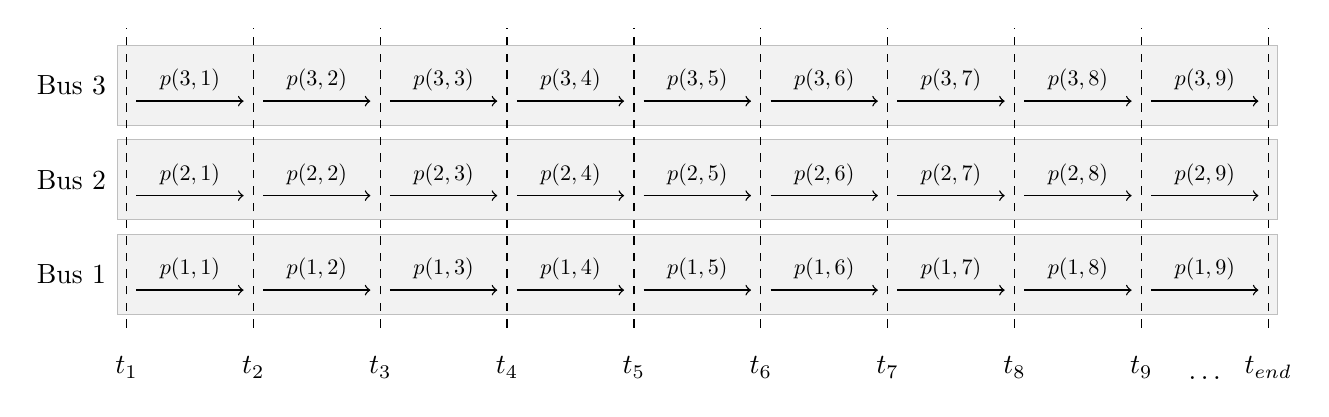
\begin{tikzpicture}
	\node[rectangle, draw=gray!50, fill=gray!10, minimum width=5.8in, minimum height=0.4in](bus1Box) at (7.75,0.8){};
	\node(bus1BoxLabel) at (-0.2, 0.8){Bus 1}; 
	
	\node[rectangle, draw=gray!50, fill=gray!10, minimum width=5.8in, minimum height=0.4in](bus2Box) at (7.75,2){};
	\node(bus1BoxLabel) at (-0.2, 2.0){Bus 2};
	
	\node[rectangle, draw=gray!50, fill=gray!10, minimum width=5.8in, minimum height=0.4in](bus3Box) at (7.75,3.2){};
	\node(bus1BoxLabel) at (-0.2, 3.2){Bus 3};
	
	\foreach \curLab/\preLab[count=\c, evaluate=\c as \pos using {0.5 + (\c - 1)*14.5/9}] in {t_1/t_1, t_2/t_1, t_3/t_2, t_4/t_3, t_5/t_4, t_6/t_7, t_7/t_6, t_8/t_7, t_9/t_8, t_{end}/t_9}
	{
		\node[label=below:$\curLab$](b\c) at (\pos, 0){};
		\node(t) at (\pos, 3.8){};
		\draw[dashed, line width=0.5pt] (b\c.north) -- (t.north); 
		\ifnum\c>1 
			\node(b1Curr) at (\pos, 0.8 - 0.2){};
			\node(b2Curr) at (\pos, 2.0 - 0.2){};
			\node(b3Curr) at (\pos, 3.2 - 0.2){};
			\def\temp{\number\numexpr\c - 1}
			\draw[->, line width=0.5pt] (b1Prev.east) -- node[midway, above]{\scalebox{0.8}{$p(1,\temp)$}}(b1Curr.west);
			\draw[->, line width=0.5pt] (b2Prev.east) -- node[midway, above]{\scalebox{0.8}{$p(2,\temp)$}}(b2Curr.west);
			\draw[->, line width=0.5pt] (b3Prev.east) -- node[midway, above]{\scalebox{0.8}{$p(3,\temp)$}}(b3Curr.west);	
		\fi
			\node(b1Prev) at (\pos, 0.8 - 0.2){};
			\node(b2Prev) at (\pos, 2.0 - 0.2){};
			\node(b3Prev) at (\pos, 3.2 - 0.2){};	
	}
	\path (b9.south) -- node[midway, below=0.1in]{$\hdots$}(b10.south);

\end{tikzpicture}}
\caption{Demonstrates how bus power use is conceptualized}
\label{fig:busPower}
\end{figure*}


\begin{figure*}
\centering
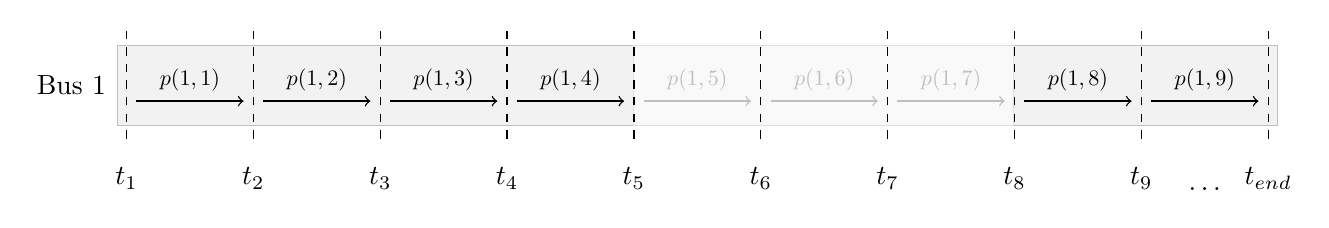
\begin{tikzpicture}
	\node[rectangle, draw=gray!50, fill=gray!10, minimum width=5.8in, minimum height=0.4in](bus1Box) at (7.75,0.8){};
	\node(bus1BoxLabel) at (-0.2, 0.8){Bus 1}; 
	\node[rectangle, draw=gray!25, fill=gray!5, minimum width=1.9in, minimum height=0.4in](bus1Box) at (7.75 + 1.6,0.8){};
	
	\foreach \curLab/\preLab[count=\c, evaluate=\c as \pos using {0.5 + (\c - 1)*14.5/9}] in {t_1/t_1, t_2/t_1, t_3/t_2, t_4/t_3, t_5/t_4, t_6/t_5, t_7/t_6, t_8/t_7, t_9/t_8, t_{end}/t_9}
	{
		\node[label=below:$\curLab$](b\c) at (\pos, 0){};
		\node(t) at (\pos, 1.4){};
		\ifnum\c>1 
			\node(b1Curr) at (\pos, 0.8 - 0.2){};
				\ifnum\c > 5
					\ifnum\c < 9 
						\def\clr{black!25}
					\else
						\def\clr{black}
					\fi
				\else
					\def\clr{black}
				\fi
				\draw[->, line width=0.5pt, \clr] (b1Prev.east) -- node[midway, above]{\scalebox{0.8}{$p(1,\number\numexpr\c-1)$}}(b1Curr.west); 
		\fi
		\node(b1Prev) at (\pos, 0.8 - 0.2){};
		\draw[dashed, line width=0.5pt] (b\c.north) -- (t.north); 
	}
	\path (b9.south) -- node[midway, below=0.1in]{$\hdots$}(b10.south);

\end{tikzpicture}
\caption{Bus schedule with availability}
\label{fig:busAvail}
\end{figure*}

 
\subsection{Formulation \label{sec:formulation}} 
The cost objective we minimize is based on the rate schedule from \cite{rocky_mountain_power_rocky_2021}, which contains two primary elements: the cost of energy, and power demand. Energy is billed per kWh for on-peak and off-peak hours. The on-peak rate is more expensive because there is generally more demand for power during this time, whereas off-peak hours tend to be less expensive. The demand is covered in two separate chargers.  The first is a facilities charge which is billed per kW for the highest 15-minute average power use over the course of the month. The second is a demand charge, which is also billed per kW, but is only billed for the highest 15-minute average power usesd during on-peak hours. The rates for each component are given in Table \ref{tab:charges}.  

Before we may compute the total monthly cost of electricity, we must define expressions for the average power and energy over time.  Let each day be divided into time intervals of length $\Delta T$ for each bus where the average power expended for bus $i$ during time $j$ is denoted $p(i,j)$ as shown in Fig. \ref{fig:busPower} (Note that $\Delta T$ may not be 15 minutes, and expressions for the 15-minute average will be computed later). The resulting solution of $p_1$ will yield the average power expended by each bus during each period of time.
\par One constraint for which the solution must account is bus availability.  When a bus is out of the station, the maximum average power for that time must be zero. For example, if bus 1 were out on route for $t_5, t_6,$ and $t_7$, then the average power for those periods would be equal to zero as shown in Fig. \ref{fig:busAvail}. Let $\bm{b}_{p(i,j)}$ be the average power used by bus $i$ at time index $j$, and $\bm{b}$ be a vector which contains $b_{p(i,j)}$ for each bus and time index. Also let $\mathcal{A} \subset {i\times j}$  be the set of all indices where bus $i$ is in the station during time $t_j$ and $\tilde{\mathcal{A}}$ be its complement. Furthermore, let $p_{\text{max}}$ be the maximum power that a charger can deliver. 
\par We define a set of constraints so that buses do not use power when not in the station by letting
\begin{equation}\label{eqn:obj:power2}\begin{aligned}
	b_{p(i,j)} &= 0 \ \forall i,j \in \tilde{\mathcal{A}}  \\
	b_{p(i,j)} &\le p_{\text{max}} \ \forall i,j \in \mathcal{A} \\
	-b_{p(i,j)} &\le 0              \ \forall i,j \in \mathcal{A} 
\end{aligned}\end{equation}


\subsection{Battery}
\par Each bus must also maintain its state of charge above acceptable levels throughout the day.  When buses leave the station, each bus discharges some quantity of energy throughout the course of the route. Let $\delta(i,j)$ be the amount of charge lost by bus $i$ at time $j$ and let $h(i,j)$ be the state of charge of bus $i$ at time $j$. The state of charge for each bus can be defined as
\begin{equation}\label{eqn:battery:socPropagation}\begin{aligned}
	h(i,j) &= h(i,j-1) + b_p(i,j - 1)\cdot \Delta T - \delta(i,j) \ \forall i,j>1 \\
	h(i,1) &= \eta_i \ \forall i
\end{aligned}\end{equation}
where $\eta_i$ is the initial state of charge for bus $i$ and $\Delta T$ is the difference in time between $t_{i,j}$ and $t_{i,j+1}$.
Now that each value for the state of charge is defined, each value for $h$ must be constrained so that it is greater than a given threshold, $h_{\text{min}}$ but does not exceed the maximum battery capacity $h_{\text{max}}$. This yields
\begin{equation} \label{eqn:battery:soc}\begin{aligned}
	-h(i,j) &\le -h_{\text{min}}\ \forall i,j \\
	h(i,j) &\le h_{\text{max}} \ \forall i,j. 
\end{aligned}\end{equation}
\par The final battery related constraint has to do with how we are planning for the bus.  The expenses that come from power are computed monthly, but we desire to simulate the movements of the bus for only a day, and use this to extrapolate what the monthly cost may be.  Therefore, the state of charge for a bus at the end of the day must reflect its starting value.  This yields the following constraint:
\begin{equation}\label{eqn:battery:busPower}
	h_{i,\text{end}} = h(i,1) \ \forall i.
\end{equation}


\subsection{Cumulative Load Management}
\par While this formulation does not directly account for the number of available chargers, we do account for the cumulative load capacities of all chargers.  Let the number of chargers be denoted $n_{\text{charger}}$. We desire to maintain the average cumulative power for each time step at a level that is serviceable given $n_{\text{charger}}$. We define a slack variable $p_c(j)$ which represents the total average power consumed by all buses at time $j$.  The variable $p_c(j)$ is computed as the sum of average bus powers so that
\begin{equation}\label{eqn:cumulative:power}
	p_c(j) = \sum_ib_{p(i,j)}.
\end{equation}

\subsection{Objective\label{sec:objective}}

\par Now that the relevent constraints have been addressed, we turn attention to the objective function. We start by computing the total average power for the complete system. This total power is comprised of power used by the buses, and power used by external sources such as lights, ice melt, electric trains, etc which we refer to as ``uncontrolled loads'', where the average power for the uncontrolled loads at time step $j$ is denoted $u(j)$. We compute the total power as the sum of power used by the buses, $p_c(j)$ and the power consumed by uncontrolled loads $u(j)$ so that the total power, denoted $p_t(j)$ is computed as 
\begin{equation}\label{eqn:objective:pt}
	p_t(j) = p_c(j) + u(j).
\end{equation}
      
\par The next step is to compute the fifteen minute average power use for each time step, denoted $p_{\text{15}}$. We do this by letting 
\begin{equation}\label{eqn:objective:p15}
p_{\text{15}}(j) = \frac{1}{n}\sum_{l \in \{j_{15}\}}p_t(l)
\end{equation}
where $\{j_{15}\}$ is the set of all indices 15 minutes prior to time $t_j$ and $n$ is the cardinality of $\{j_{15}\}$.
Next, note that the rate schedule requires both the maximum overall average power, denoted $p_{\text{facilities}}$, and the maximum average power during on-peak hours, or $p_{\text{demand}}$. Let $\mathcal{S}_{\text{on}}$ be the set of time indices belonging to on-peak hours, and recall that the max over all average power values is greater than or equal to $p_{15}(j)$ for all $j$. We can express this constraint as
\begin{equation}\label{eqn:objective:pFac}
	p_{\text{facilities}} \ge p_{15}(j) \ \forall j.
\end{equation}
Because $p_{\text{facilities}}$ will be used in the objective function, the value for $p_{\text{facilities}}$ will be minimised until it is equal to the largest value in $p_{15}$. Following a similar logic, we also define a set of constraints for the maximum average on-peak power, $p_{\text{demand}}$ so that
\begin{equation}\label{eqn:objective:pDem}
	p_{15}(i) \leq p_{\text{demand}} \ \forall i \in \mathcal{S}_{\text{on}}.
\end{equation}
The next step in computing the objective function is to compute the total {\it energy} consumed during on and off-peak hours respectively.  Let $e_{\text{on}}$ be the total energy consumed during on-peak hours and $e_{\text{off}}$ be the energy consumed during off-peak hours. We can compute energy as the product of average power and time.  In our case, we compute this as 
\begin{equation}\label{eqn:objective:energy}\begin{aligned}
	e_{\text{on}} &= \Delta T\cdot \sum_{i \in \mathcal{S}_{\text{on}}}p_t(i) \\ 
	e_{\text{off}} &= \Delta T\cdot \sum_{i \notin \mathcal{S}_{\text{on}}}p_t(i).  
\end{aligned}\end{equation}
We can now compute the total monthly cost in dollars as
\begin{equation}\label{sec:unconstrainedSchedule:objective}
J_{\text{cost}} = \begin{bmatrix}e_{\text{on}} \\ e_{\text{off}} \\ p_{\text{facilities}} \\ p_{\text{demand}} \end{bmatrix}^T \begin{bmatrix} \mu_{\text{e-on}} \\ \mu_{\text{e-off}} \\ \mu_{\text{p-all}} \\ \mu_{\text{p-on}} \end{bmatrix} 
\end{equation}

\par The final optimization problem that computes a charge schedule without constraints on the number of chargers is descibed below.\\[0.1in]
\begin{tikzpicture}
	\node[rectangle, rounded corners, fill=gray!8, draw=gray!60, minimum width=\columnwidth, minimum height=0.7in] at (0,0)(box){};
	\node at (0,0.2in)(title){\underline{Summary for $P_1$}};
	\node at ($(box.south)!0.6!(title.south)$)(text){$ 
	\underset{\mathbf{y}}{\text{Min}}  \ \eqref{sec:unconstrainedSchedule:objective} \  \text{subject to} \ \eqref{eqn:obj:power2} \ \text{--} \ \eqref{eqn:objective:energy}.% \ \eqref{eqn:battery:socPropagation}, \ \eqref{eqn:battery:soc}, \ \eqref{eqn:battery:busPower}, \ \eqref{eqn:cumulative:power}, \ \eqref{eqn:objective:pt}, \ \eqref{eqn:objective:p15}, \ \eqref{eqn:objective:pFac}, \ \eqref{eqn:objective:pDem}, \ \eqref{eqn:objective:energy}
$};
\end{tikzpicture}

\par We have observed that charge commands in solutions to $P_1$ tend to switch frequently between $0$ and $p_{\text{max}}$, which is difficult to implement in practice and imparts stress on charging hardware. Before additional steps can be taken, a smoother set of charge commands is computed, and this is the subject of the next section.

\section{$P_2$: Unconstrained Smooth Schedule \label{sec:unconstrainedSmoothSchedule}}

\par This section implements a smoothing criteria so that the frequent ``on-off'' switching patterns from $P_1$ are reduced. This is done by modifying $P_1$ in two ways. The first is that the demand, facilities, on-peak energy, and off-peak energy are removed from the objective and constrained to equal their values obtained in the solution to $P_1$ so that
\begin{equation}\label{eqn:unconstrainedSmooth:equivalence}\begin{aligned}
	e_{\text{on}} &= \tilde{e}_{\text{on}} \\
	e_{\text{off}} &= \tilde{e}_{\text{off}} \\
	p_{\text{facilities}} &= \tilde{p}_{\text{facilities}} \\
	p_{\text{demand}} &= \tilde{p}_{\text{demand}},
\end{aligned}\end{equation}
where values on the right-hand side are constants extracted from the solution to $P_1$.
Next, we define an alternative objective that incentivizes continuity of charging between time steps. This objective is defined as
\begin{equation}\label{eqn:objective:smooth}
	J_{\text{switch}} = \frac{1}{n}\sum_{i,j, \in \mathcal{K}}\lVert b(i,j) - b(i,j-1) \rVert^2_2,
\end{equation}
where $\mathcal{K}$ is the set of all $i,j$ where bus $i$ may charge during time $j$ and $j - 1$.  The final optimization problem that produces smooth charging schedules is given below.\\[0.1in]
\begin{tikzpicture}
	\node[rectangle, rounded corners, fill=gray!8, draw=gray!60, minimum width=\columnwidth, minimum height=0.7in] at (0,0)(box){};
	\node at (0,0.2in)(title){\underline{Summary for $P_2$}};
	\node at ($(box.south)!0.6!(title.south)$)(text){$ 
	\underset{\mathbf{y}}{\text{Min}} \ \eqref{eqn:objective:smooth} \ \text{Subject to} \ \eqref{eqn:obj:power2} \ \text{--} \ \eqref{eqn:objective:energy}, \ \eqref{eqn:unconstrainedSmooth:equivalence}
$};
\end{tikzpicture}

\par The solution to $P_2$ smooths charge schedules without increasing costs, but it presents the undesireable feature that the charge sessions tend to be fragmented into many short sessions. Additionally, the schedule does not account for the number of chargers or bus contention for charger use. Unfortunatly, addressing these problems requires the use of binary variables and optimization with binary variables becomes untractable for large numbers of buses and chargers. Before the fragmentation and charger assignment problems can be addressed, we first segment the buses into groups.  Successive processing can be done separately in groups which helps to manage the computational complexity for later problems that incorporate binary variables.

\section{$P_3$: Group Assignment\label{sec:groupAssignment}}
This section addresses the matter of problem size.  An optimization problem for scheduling must evaluate all possible combinations of bus-to-charger assignments to select an optimal, contention-free schedule. Because contention increases on the order of $O(n^2)$ with the number $n$ of charge sessions and requires that each combination be evaluated to find an optimal solution, the assignment problem is NP-hard \cite{kolesar_branch_1967}. {\textbf [I don't think $n^2$ is NP-hard.  It's just hard.]} Before we can formulate a scalable solution to the bus problem, we propose a method to separate buses into groups to reduce the coupling between charge sessions.
\par The group assignment problem separates buses into $n_{\text{group}}$ groups, where group $m$ is allocated $n^m_{\text{charger}}$ chargers and $n^m_{\text{bus}}$ buses. Each group must have sufficient chargers to fill its needs and prefer buses with dissimilar schedules to better avoid contention. 
We know that the number of cross-terms in future problems will be reduced when each group has the same number of buses. Therefore, let $n^m_{\text{bus}}$ be described as
\begin{equation}\label{eqn:groups:nBusPerGroup}\begin{aligned}
	n^m_{\text{bus}} &\ge \left \lfloor \frac{n_{\text{bus}}}{n_{\text{group}}} \right \rfloor \\
	n^m_{\text{bus}} &\le \left \lceil \frac{n_{\text{bus}}}{n_{\text{group}}} \right \rceil,
\end{aligned}\end{equation}
where the values $n_\text{bus}$ and $n_\text{group}$ are user parameters.
\par The number of chargers assigned to each group must be exactly equal to the number of available chargers so that
\begin{equation}\label{eqn:groups:nTotalCharger}
	n_{\text{charger}} = \sum_mn_{\text{charger}}^m.
\end{equation}
\par The next set of constraints ensures that each bus is is part of a group exactly once. Let $\beta(i,m)$ be a binary variable which is one when bus $i$ is in group $m$. Each bus is constrained to be a member of exactly one group by letting
\begin{equation}\label{eqn:groups:groupId}
	\sum_m\beta(i,m) = 1 \ \forall i.
\end{equation}
\par We must also ensure that buses are assigned to groups where the power delivered to each bus can be achieved with the number of chargers assigned to that group. Define a slack variable that gives the total power used in group $m$ at time step $j$ as $p(m,j)$. Recall, we also know the expected power use for each bus as this is a result of $P_1$ as $b_{p(i,j)}$, which allows us to describe the total power for any one group as
\begin{equation}\label{eqn:groups:groupPower}
 p(m,j) = \sum_i\beta(i,m)b_{p(i,j)}.
\end{equation}
\par Next, we know that the total load of each group must be less than or equal to the collective capability of that group's chargers, which can be expressed as
\begin{equation}\label{eqn:groups:chargeLimit}
	n^m_{\text{charger}}\cdot p_{\text{max}} \ge p(m,j) \ \forall m,j
\end{equation}
so that the number of chargers is sufficient to charge the collective load of the group. 
\par We also desire to group together buses whos routes have the least overlap. If two buses contain no overlap, they will be easiest to schedule on the same charger.  The overlap is measured using the inner product of their schedules from $P_1$.  If completely non-overlapping, the inner product will be equal to zero. Let
\begin{equation*}
\phi(i,i') = \mathbf{b}(i,:)^T\mathbf{b}(j,:),
\end{equation*}
where $\mathbf{b}(i,:)$ is the charge schedule for bus $i$ as computed in the $P_1$. We desire to minimize the total cross terms $\phi(i,i')$ for all buses in the same group.  Define a slack variable $v(i,i',m)$ which is equal to $\phi(i,i')$ if buses $i$ and $i'$ are both in group $m$ and zero otherwise so that
\begin{equation*}
	\begin{cases}
		v(i,i',m) = \phi(i,i') & \beta(i,m) = 1, \beta(i',m) = 1 \\
		v(i,i',m) = 0 & \text{otherwise}
	\end{cases}
\end{equation*}
which can also be expressed by letting
\begin{equation}\label{eqn:groups:innerProd}\begin{aligned}
	v(i,i',m) &\le \phi(i,i') \\
	v(i,i',m) &\ge \phi(i,i') - M\left (2 - \beta(i,m) - \beta(i',m)\right ) \\
	v(i,i',m) &\le 0 + M\beta(i,m) \\
	v(i,i',m) &\le 0 + M\beta(i',m) \\
	v(i,i',m) &\ge 0.
\end{aligned}\end{equation}
The final objective can then be expressed as
\begin{equation}\label{eqn:groups:objective}
	J_{\text{select}} = \sum_{i,i',m} v(i,i',m).
\end{equation}
The final optimization problem may be expressed as shown below. \\[0.1in]
\begin{tikzpicture}
	\node[rectangle, rounded corners, fill=gray!8, draw=gray!60, minimum width=\columnwidth, minimum height=0.7in] at (0,0)(box){};
	\node at (0,0.2in)(title){\underline{Summary for $P_3$}};
	\node at ($(box.south)!0.6!(title.south)$)(text){$ 
	\underset{\mathbf{y}}{\text{Min}} \ \eqref{eqn:groups:objective} \ \text{subject to} \ \eqref{eqn:groups:nBusPerGroup} \ \text{--} \ \eqref{eqn:groups:innerProd} % \ \eqref{eqn:groups:nTotalCharger}, \ \eqref{eqn:groups:groupId}, \ \eqref{eqn:groups:groupPower}, \ \eqref{eqn:groups:chargeLimit}, \ \eqref{eqn:groups:innerProd}
$};
\end{tikzpicture}
\par Problems $P_1$ through $P_3$ have produced preliminary estimates for charge schedules as well as groups into which the buses can be subdivided but have not addressed the problem of fragmentation, where each bus's schedule contains many short charge sessions, whereas fewer charge sessions is desirable. Before we can address where buses should charge, we must first finalize each bus's charge schedule by decreasing the number of charge events.

% imports
\begin{figure*}
\centering
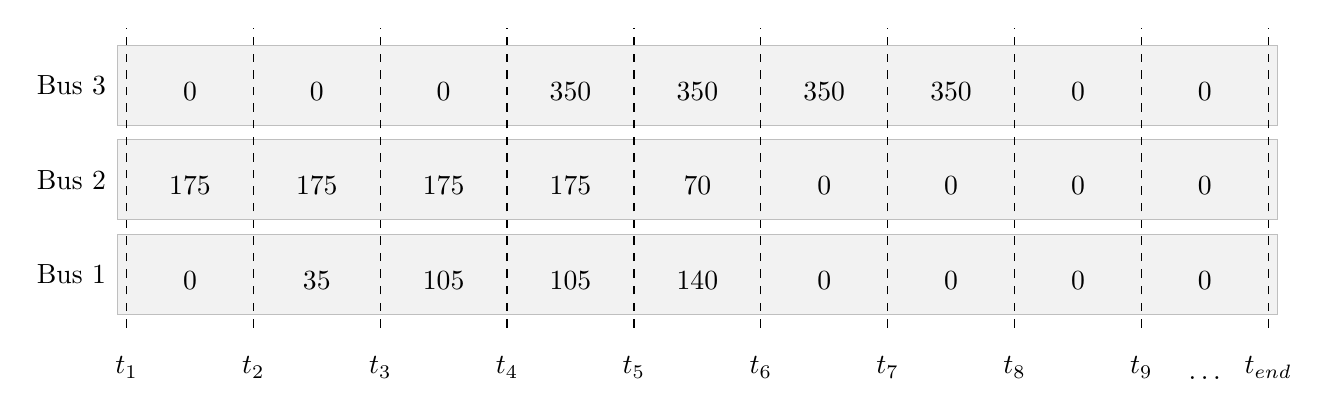
\begin{tikzpicture}
	\node[rectangle, draw=gray!50, fill=gray!10, minimum width=5.8in, minimum height=0.4in](bus1Box) at (7.75,0.8){};
	\node(bus1BoxLabel) at (-0.2, 0.8){Bus 1}; 
	
	\node[rectangle, draw=gray!50, fill=gray!10, minimum width=5.8in, minimum height=0.4in](bus2Box) at (7.75,2){};
	\node(bus1BoxLabel) at (-0.2, 2.0){Bus 2};
	
	\node[rectangle, draw=gray!50, fill=gray!10, minimum width=5.8in, minimum height=0.4in](bus3Box) at (7.75,3.2){};
	\node(bus1BoxLabel) at (-0.2, 3.2){Bus 3};
	
	\foreach \curLab/\preLab[count=\c, evaluate=\c as \pos using {0.5 + (\c - 1)*14.5/9}] in {t_1/t_1, t_2/t_1, t_3/t_2, t_4/t_3, t_5/t_4, t_6/t_7, t_7/t_6, t_8/t_7, t_9/t_8, t_{end}/t_9}
	{
		\node[label=below:$\curLab$](b\c) at (\pos, 0){};
		\node(t) at (\pos, 3.8){};
		\draw[dashed, line width=0.5pt] (b\c.north) -- (t.north); 
		\ifnum\c>1 
			\node(b1Curr) at (\pos, 0.8 - 0.2){};
			\node(b2Curr) at (\pos, 2.0 - 0.2){};
			\node(b3Curr) at (\pos, 3.2 - 0.2){};
			\path(b1Prev.east) -- node(node1\c)[midway, above]{}(b1Curr.west);
			\path(b2Prev.east) -- node(node2\c)[midway, above]{}(b2Curr.west);
			\path(b3Prev.east) -- node(node3\c)[midway, above]{}(b3Curr.west);	
		\fi
			\node(b1Prev) at (\pos, 0.8 - 0.2){};
			\node(b2Prev) at (\pos, 2.0 - 0.2){};
			\node(b3Prev) at (\pos, 3.2 - 0.2){};	
	}
	\path (b9.south) -- node[midway, below=0.1in]{$\hdots$}(b10.south);
	\node at (node12.center){0};
	\node at (node13.center){35};
	\node at (node14.center){105};
	\node at (node15.center){105};
	\node at (node16.center){140};
	\node at (node17.center){0};
	\node at (node18.center){0};
	\node at (node19.center){0};
	\node at (node110.center){0};
	\node at (node22.center){175};
	\node at (node23.center){175};
	\node at (node24.center){175};
	\node at (node25.center){175};
	\node at (node26.center){70};
	\node at (node27.center){0};
	\node at (node28.center){0};
	\node at (node29.center){0};
	\node at (node210.center){0};
	\node at (node32.center){0};
	\node at (node33.center){0};
	\node at (node34.center){0};
	\node at (node35.center){350};
	\node at (node36.center){350};
	\node at (node37.center){350};
	\node at (node38.center){350};
	\node at (node39.center){0};
	\node at (node310.center){0};

\end{tikzpicture}
\caption{An example solution to a 3-bus, 2-charger scenario from the first QP}
\label{fig:solutionExample}
\end{figure*}

\begin{figure*}
\centering
\scalebox{0.8}{
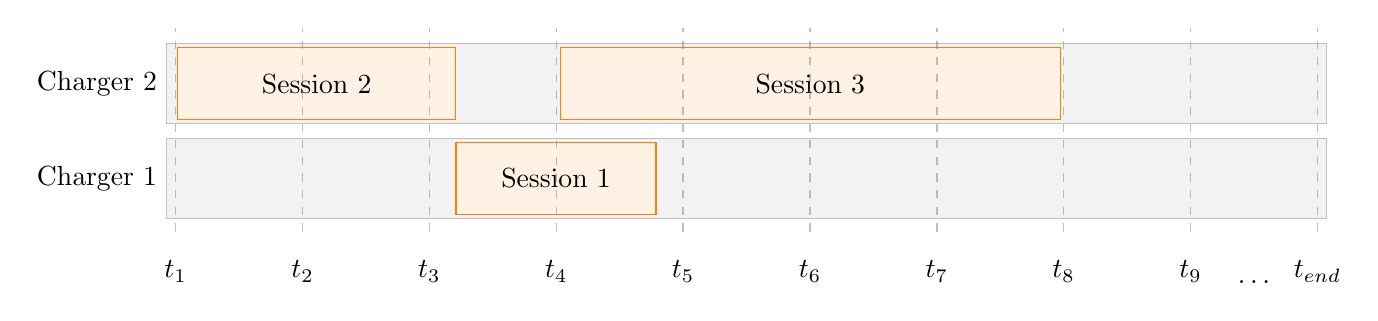
\begin{tikzpicture}
	\node[rectangle, draw=gray!50, fill=gray!10, minimum width=5.8in, minimum height=0.4in](bus1Box) at (7.75,0.8){};
	\node(bus1BoxLabel) at (-0.5, 0.8){Charger 1}; 

	\node[rectangle, draw=gray!50, fill=gray!10, minimum width=5.8in, minimum height=0.4in](bus2Box) at (7.75,2){};
	\node(bus1BoxLabel) at (-0.5, 2.0){Charger 2};
	\node[rectangle, draw=orange!100, fill=orange!10, minimum width=1.3915in, minimum height=0.36in](charge111) at (2.29, 2){Session 2}; 
	\node[rectangle, draw=orange!100, fill=orange!10, minimum width=1in, minimum height=0.36in](charge111) at (5.33, 0.8){Session 1};
	\node[rectangle, draw=orange!100, fill=orange!10, minimum width=2.50in, minimum height=0.36in](charge111) at (8.56, 2){Session 3};


	\foreach \curLab/\preLab[count=\c, evaluate=\c as \pos using {0.5 + (\c - 1)*14.5/9}] in {t_1/t_1, t_2/t_1, t_3/t_2, t_4/t_3, t_5/t_4, t_6/t_7, t_7/t_6, t_8/t_7, t_9/t_8, t_{end}/t_9}
		{
			\node[label=below:$\curLab$](b\c) at (\pos, 0){};
			\node(t) at (\pos, 2.58){};
			\draw[dashed, line width=0.5pt, black!50, opacity=0.5] (b\c.north) -- (t.north); 
		}
		\path (b9.south) -- node[midway, below=0.1in]{$\hdots$}(b10.south); 
\end{tikzpicture}}
\caption{Demonstrates the solution to $p_5$}
\label{fig:secondSolutionExample}
\end{figure*}



\begin{figure*}
\centering
\scalebox{0.8}{
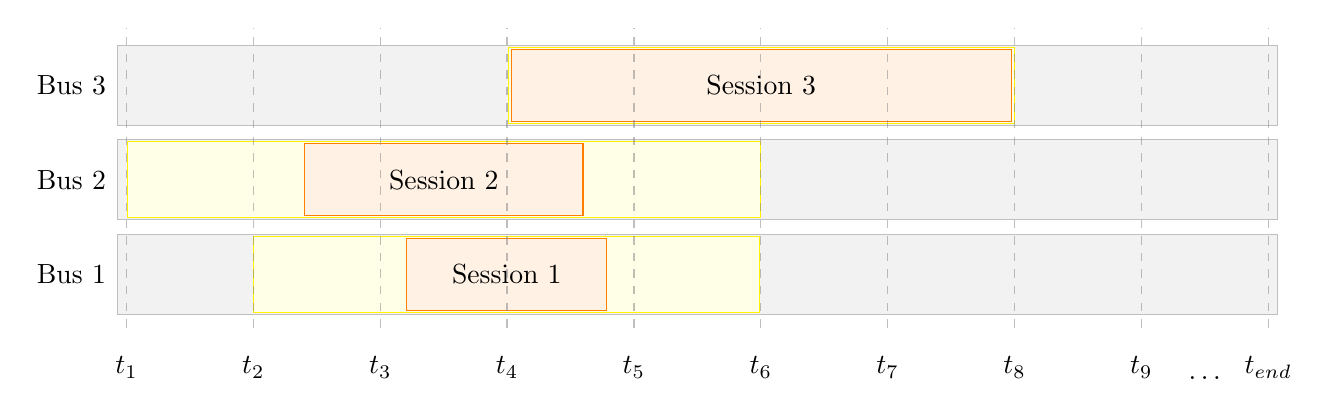
\begin{tikzpicture}
	\node[rectangle, draw=gray!50, fill=gray!10, minimum width=5.8in, minimum height=0.4in](bus1Box) at (7.75,0.8){};
	\node(bus1BoxLabel) at (-0.2, 0.8){Bus 1}; 
	\node[rectangle, draw=yellow!100, fill=yellow!10, minimum width=2.53in, minimum height=0.38in](charge11) at (5.33, 0.8){};
	\node[rectangle, draw=orange!100, fill=orange!10, minimum width=1in, minimum height=0.36in](charge111) at (5.33, 0.8){Session 1};

	\node[rectangle, draw=gray!50, fill=gray!10, minimum width=5.8in, minimum height=0.4in](bus2Box) at (7.75,2){};
	\node(bus1BoxLabel) at (-0.2, 2.0){Bus 2};
	\node[rectangle, draw=yellow!100, fill=yellow!10, minimum width=3.1625in, minimum height=0.38in](charge11) at (4.53, 2){};
	\node[rectangle, draw=orange!100, fill=orange!10, minimum width=1.3915in, minimum height=0.36in](charge111) at (4.53, 2){Session 2};
	
	\node[rectangle, draw=gray!50, fill=gray!10, minimum width=5.8in, minimum height=0.4in](bus3Box) at (7.75,3.2){};
	\node(bus1BoxLabel) at (-0.2, 3.2){Bus 3}; 
	\node[rectangle, draw=yellow!100, fill=yellow!10, minimum width=2.53in, minimum height=0.38in](charge11) at (8.56, 3.2){};
	\node[rectangle, draw=orange!100, fill=orange!10, minimum width=2.50in, minimum height=0.36in](charge111) at (8.56, 3.2){Session 3};


	\foreach \curLab/\preLab[count=\c, evaluate=\c as \pos using {0.5 + (\c - 1)*14.5/9}] in {t_1/t_1, t_2/t_1, t_3/t_2, t_4/t_3, t_5/t_4, t_6/t_7, t_7/t_6, t_8/t_7, t_9/t_8, t_{end}/t_9}
		{
			\node[label=below:$\curLab$](b\c) at (\pos, 0){};
			\node(t) at (\pos, 3.8){};
			\draw[dashed, line width=0.5pt, black!50, opacity=0.5] (b\c.north) -- (t.north); 
		}
		\path (b9.south) -- node[midway, below=0.1in]{$\hdots$}(b10.south); 
\end{tikzpicture}}
\caption{Demonstrates how results from $p_4$ can be reexpressed in terms of continuous variables} 
\label{fig:refactorExample}
\end{figure*}



\begin{figure*}
\centering
\scalebox{0.8}{
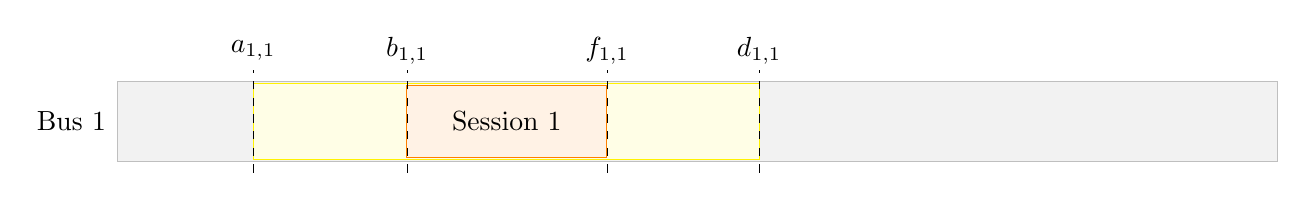
\begin{tikzpicture}
	\node[rectangle, draw=gray!50, fill=gray!10, minimum width=5.8in, minimum height=0.4in](bus1Box) at (7.75,0.8){};
	\node(bus1BoxLabel) at (-0.2, 0.8){Bus 1}; 
	\node[rectangle, draw=yellow!100, fill=yellow!10, minimum width=2.53in, minimum height=0.38in](charge11) at (5.33, 0.8){};
	\node[rectangle, draw=orange!100, fill=orange!10, minimum width=1in, minimum height=0.36in](charge111) at (5.33, 0.8){Session 1}; 
	\draw[dashed] (0.83in,0.15) -- (0.83in,1.45);
	\node at (0.83in,1.7){$a_{1,1}$};
	\draw[dashed] (3.36in, 0.15) -- (3.36in, 1.45);
	\node at (3.36in,1.7){$d_{1,1}$};
	\draw[dashed] (1.6in, 0.15) -- (1.6in, 1.45);
	\node at (1.6in,1.7){$b_{1,1}$};
	\draw[dashed] (2.6in, 0.15) -- (2.6in, 1.45);
	\node at (2.6in,1.7){$f_{1,1}$};
\end{tikzpicture}}
\caption{Gives variables of optimization for $p_5$}
\label{fig:secondProgramVars}
\end{figure*} 


\section{Charge Schedules}
The results from the Linear Program defined in the previous section give us a general estimate of how much and when buses should charge, however we must still address two primary issues. The first is defining concrete start and stop times for each charge session. The second is limiting the charge sessions to a finite number of chargers. After solving the first program, we take the results and derive {\it preliminary} intervals and average power consumptions for each charge session.  
\par For example, consider a solution to a three bus, two charger scenario given in Fig. \ref{fig:solutionExample}.
Note that there appears to be three buses charging at the same time from $t_5$ to $t_6$ even though there are only two chargers.  We can reformulate this solution in terms of continuous start and stop variables and a variable charge rate so that the {\it duration} of each charge session may be relaxed. The objective is to store the given energy in the corresponding bus within the given charge interval.  
\par Note how few of the charge sessions utilize the chargers to full capacity. This implies that there exists a smaller charge window in which equivalent power can be delivered. This allow us to use the charge durations from the solution from Fig. \ref{fig:solutionExample} as bounds on {\it allowable} charge windows instead of absolute truth. 
\par An example of how Fig. \ref{fig:solutionExample} may be reformulated is given in Fig. \ref{fig:refactorExample}. Note how the actual charge sessions don't necessarily need to take up all the time they were initially allocated in the first solution and that these times can fluctuate if the average charge rate is less than the maximum charger capacity. In this example, we assume a maximum charge capacity of 350kW.  
\par Note how the third charge session does have to be exactly where it was scheduled because the average is equal to the maximum charge rate.
If we examin just the schedule for Bus 1, we note that there are four essential variables for the corresponding charge session: $a(i,r)$, $b(i,r)$, $f(i,r)$ and $d(i,r)$ which represent the minimum start time, actual start time, actual end time, and maximum end time respectively. 
\par The problem we must now solve is one of arranging these ``rectangles'' such that each one is larger than it's minimum width (or charge time).  We must also account for the number of chargers. It can be helpful to view the problem as a bin packing problem, where each session must fit within the ``swim lane'' of a charger.  For example, taking the charge sessions given in Fig. \ref{fig:refactorExample} and arranging them so that there is no overlap between sessions will yield a valid solution as shown in Fig. \ref{fig:secondSolutionExample}.
\par From Fig. \ref{fig:secondProgramVars}, we know that $a(i,r), b(i,r),f(i,r)$ and $d(i,r)$ must be such that 
\begin{equation*}\begin{aligned}
	a(i,r) \le b(i,r) \\
	b(i,r) \le f(i,r) \\
	f(i,r) \le d(i,r). 	
\end{aligned}\end{equation*}
or alternatively as
\begin{equation} \begin{aligned}
	-b(i,r) &\le -a(i,r) \\
	b(i,r) - f(i,r) &\le 0 \\
	f(i,r) &\le d(i,r)
\end{aligned} \end{equation}
Where $a(i,r)$ and $d(i,r)$ are known from the previous optimization problem, and $b(i,r)$ and $f(i,r)$ are optimization variables. 
\par We must differentiate between chargers and so, define $\sigma_{i,r,k}$ as a binary selector variable which is one if charger $k$ services bus $i$ for session $r$ and zero otherwise. We know that only one charger can charge each bus at a time. We also know that each charge session {\it must} be serviced, which implies that
\begin{equation}
	\sum_k \sigma(i,r,k) = 1  \ \forall i,r.
\end{equation}
\par Next, we also know that during each session a certain amount of energy must be transfered from the charger to the battery.  The amount of energy that must be transfered to bus $i$ during session $r$ can be computed from the results of the first linear program and is denoted $e(i,r)$. We can compute a minimum time window from this value as 
\begin{equation*}
	w(i,r)_{\text{min}} = \frac{e(i,r)}{p_\text{max}}.
\end{equation*}
\par Because this is the minimum time window, we must ensure that the difference between the start and stop times is at least this large so that
\begin{equation*}
	f(i,r) - b(i,r) \ge w(i,r) \ \forall i,r	
\end{equation*}
or alternatively,
\begin{equation}
	b(i,r) - f(i,r) \le -w(i,r) \ \forall i,r.
\end{equation}
\par The final set of constraints deals with contention so that no charger can be scheduled for two sessions that overlap. let $\mathcal{L} = \{(i,r)\times (i',r') \}$ where charge sessions $i,r$ and $i',r'$ have the potential to overlap. Before we can prevent overlap, we must define a binary variable $l(i,r,i',r')$ which is equal to one when session $i,r$ is scheduled before session $i',r'$ and zero otherwise so that
\begin{equation*}
	\begin{cases}
		f(i,r) \le b(i',r') & l(i,r,i',r') = 1 \\
		f(i',r') \le b(i',r') & l(i,r,i',r') = 0 
	\end{cases}
\end{equation*}
Here we can expand this thought through use of the ``big-M'' technique.  Let $M$ be large. In this case, we can set it equal to the number of seconds in a day. We know what the top constraint must be trivially satisfied when $l(i,r,i',r') = 0$ and the bottom must also when $l(i,r,i',r') = 1$.  This leads to a reformulation so that
\begin{equation*}\begin{aligned}
		f(i,r) - b(i',r') & \le M(1 - l(i,r,i',r')\\
		f(i',r') - b(i,r) & \le l(i,r,i',r')M  
\end{aligned}\end{equation*}
However, this constraint {\it only} needs to hold when sessions $i,r$ and $i',r'$ are scheduled to charge on the same charger or that $\sigma(i,r,k) = \sigma(i',r',k) = 1$. We can reformulate the above constraint to satisfy this condition by letting
\begin{equation}\begin{aligned}
	f(i,r) - b(i',r') & \le M(3 - \sigma(i,r,k) - \sigma(i',r',k) - l(i,r,i',r')) \\
	f(i',r') - b(i,r) & \le M(2 - \sigma(i,r,k) - \sigma(i',r',k) + l(i,r,i',r'))
\end{aligned}\end{equation}
\par Finally, we desire the power profile to closly match the profile given in the first linear program, which would occure if each charge session matched the durations given in the first solution.  We considered linear formulation such as minimimzing the absolute value of errors, or maximizing the width of the charge sessions. The problem with linear objectives is that there is nothing to balance differences between charge session. For example, one route may have a very small charge window so that the next may be very large. These small charge windows lead to high power use and are undesireable. We solve this problem by developing a quadratic loss which minimizes the squared error between the desired and given start and stop times. This leads to
\begin{equation*}
	\underset{f,b}{\text{min}} \sum_{i,r}\lVert b(i,r) - a(i,r)\rVert_2^2 + \lVert f(i,r) - d(i,r) \rVert_2^2
\end{equation*}
which has the effect of driving each variable to the desired value and more heavily penalizing values that are further from their optimal.
\begin{comment}
\par We desire to solve this second optimization method in a greedy fashion using a heuristic approach. Let $\mathcal{B}$ be the set of all charge sessions which are sorted according to their {\it latest} start time.  Begin by removing the first, or earliest, $n_{\text{charger}}$ sessions and placing them in separate queues for a charger. For the remainder of the charge sessions, we remove the next item from the list, determine which chargers are available to service this request by checking that the previous service can finish before the next will start, and then select the charger which yields the smallest amount of overlap in session availability.
\begin{algorithm}[!ht]
\DontPrintSemicolon
\KwIn{Sorted List of Charge Sessions}
\KwOut{Charge Schedule for Each Charger}
\For{i = 1:$n_{\text{charger}}$}
{
	charger[i].append(inputList.pop())
}
\While{inputList not empty}
{
	item = inputList.pop()\;
	\For{i = 1:$n_{\text{charger}}$}
	{
		bestOverlap = inf\;
		bestCharger = -1\;
		\If{charger $i$ is available}		
		{
			\If{overlap is less than bestOverlap}
			{
				bestOverlap = itemOverlap\;
				bestCharger = i\;
			}
		}
	}
	charger[bestCharger].append(item)\;
}
\caption{Pseudocode that illustrates how charge sessions are assigned}
\label{alg:chargeAssign}
\end{algorithm}
\end{comment}

\section{Multi-Rate Charging}
Up to this point, we have computed the ``optimal'' schedule which assumes any bus can charge without regard to the number of chargers. We then separate buses into groups to reduce the scope of the problem and treat each sub-problem separately while we assign them to specific chargers and determine the final start and stop times for each bus's charge session. \par At this point, Each charge session assumes the same charge rate at each time step during a session. This can lead to high instantaneous power use, especially when the number of chargers is large. In this step, we combine the results of each sub-problem from the previous step into a preliminary final solution which includes start and stop times for each charge session, charger assignments, and the average charge rate for each session. 
\par In this section, we use these results to compute a fine-tuned solution which varies the charge rate at each time step so that the power profile for the resulting solution more closely matches ``optimal'' profile given in the first linar program. Let $x(i,j)$ represent the power used for bus $i$ during timestep $j$ and $z(j)$ be the total power used by the buses at time $j$. 
\par We desire to minimize the difference between $x(i,j)$ and $p_c(i,j)$ for each $i,j$. Before we can formulate the final objective function, we must first consider constraints that preserve the information from the previous programs which includes both the energy delivered per session, and each session's start and stop times.
\par First, define $\gamma(i,d)$ as a $n_{\text{time}}\times 1$ vector which is one when bus $i$ is scheduled to charge for charge session $d$. We assume $\gamma(i,d)$ to be known as these values can be infered from the original start and stop times given in the third program.  The variable $\gamma(i,d)$ can be used to enforce the energy constraints so that
\begin{equation}
	\gamma(i,d)'x(i,:) = e(i,d) \ \forall i,d
\end{equation}
where $x(i,:)$ is the optimization variable for this problem that relates to the charge schedule for bus $i$ and $e(i,d)$ is the required energy for charge session $i,d$.
\par The next constraint is used to compute the total power used by all buses per time interval, $z(j)$ so that
\begin{equation*}
	z(j) = \sum_ix(i,j) \ \forall j	
\end{equation*}
or alternatively in standard form as 
\begin{equation*}
	z(j) - \sum_ix(i,j) = 0\ \forall j.
\end{equation*}
\par Now that each variable has been defined, we give the loss function as the squared difference between the charge profile $z(j)$ and the optimal schedule $p_c(j)$ so that
\begin{equation}
	J_{\text{multi-rate}} = \sum_i \lVert p_c(j) - z(j) \rVert_2^2
\end{equation}


%\input{11_future.tex}
%\input{8_results.tex}
%\input{9_future.tex}
\section*{Acknowledgment}This material is based in part upon work supported by the National Science Foundation through the ASPIRE Engineering Research Center under Grant No. EEC-1941524, the Department of Energy through a prime award with ABB under Grant No. DE-EE0009194, and PacifiCorp under contract number 3590. Any opinions, findings, and conclusions or recommendations expressed in this material are those of the authors and do not necessarily reflect the views of the National Science Foundation, the Department of Energy, or Pacificorp.
%\newpage 
\input{10_bigasstable.tex}
\printbibliography
\end{document}


